\documentclass[11pt]{report}
\usepackage{amsmath}
\usepackage{amssymb}
%\usepackage{bbm}
\usepackage{graphicx}
\usepackage{tikz}

\newcommand{\ubt}[1]{\textbf{\underline{#1}}}
\newcommand{\sps}{\\[0.2cm]}
\newcommand{\spn}[1]{\\[#1cm]}
\newcommand{\refn}[1]{(\ref{#1})}
\newcommand{\refx}[1]{\refn{eq:#1}}
\newcommand{\bt}[1]{\textbf{#1}}
\newcommand{\zbar}{\overline{z}}
\newcommand{\sprime}{'}
\newcommand{\dprime}{''}
\newcommand{\tprime}{'''}
\newcommand{\dsp}{\displaystyle}
\newcommand{\NI}{\noindent}
\newcommand{\real}{ \mathbb{R}}
\newcommand{\imaginary}{\imath}
\newcommand{\mbf}[1]{\mathbf{#1}}
\newcommand{\complex}{\mathbb{C}}
\newcommand{\Laplace}{\mathcal{L}}
\newcommand{\sbracket}[1]{\left[#1\right]}
\newcommand{\example}[1]{\section*{\ubt{Example #1}}}
%\newcommand{\definition}[1]{\Large{\NI\ubt{Defintion}~~\bt{#1:}}}
\newcommand{\solution}{\subsubsection{\ubt{Solution}}}

\newtheorem{theorem}{Theorem}[section]
\newtheorem{definition}{Definition}[section]
\newtheorem{corollary}{Corollary}[section]


%\newcommand{\real}{\mathbbm{R}}

\renewcommand{\baselinestretch}{1.5}
\renewcommand{\contentsname}{Table of Contents}
%\renewcommand{\labelenumi}{\roman{enumi}.}


%\setlength{\parindent}{1em}


\begin{document}
	
	%%%%%%%%%%%%%%%%%%%FRONT COVER%%%%%%%%%%%%%%%%%%%
	\addcontentsline{toc}{chapter}{TITLE PAGE}
	\clearpage
	\thispagestyle{empty}
	\begin{center}
		\Large \bt{LAURENT SERIES OF COMPLEX-VALUED FUNCTIONS AND APPLICATIONS}
	\end{center}

	\hspace{7cm}
	
	\begin{center}
		\textbf{\textit{BY}}
	\end{center}
	
	\hspace{5cm}
	
	\begin{center}
		\large \textbf{ADEGOKE, AANUOLUWAPO ABIODUN
			\\
			17/30GD007}
	\end{center}
	
	\hspace{9cm}
	
	\begin{center}
		A PROJECT SUBMITTED TO THE DEPARTMENT OF MATHEMATICS, FACULTY OF PHYSICAL SCIENCES, UNIVERSITY OF ILORIN, ILORIN, KWARA STATE, NIGERIA.
	\end{center}

	\hspace{7cm}
	
	\begin{center}
		IN PARTIAL FULFILLMENT OF REQUIREMENTS FOR THE AWARD OF BACHELOR OF SCIENCE (B. Sc.) DEGREE IN MATHEMATICS.
	\end{center}
	\hspace{5cm}
	\\ \\ 
	\begin{center}
		\textbf{November, 2022}
	\end{center}

	\newpage
	\pagenumbering{roman}
	\addcontentsline{toc}{chapter}{CERTIFICATION}
	\section*{\begin{center}\textbf{\Large CERTIFICATION}   \end{center}}
	This is to certify that this project was carried out by \textbf{ADEGOKE, Aanuoluwapo Abiodun} with Matriculation Number  17/30GD007 in the Department of Mathematics, Faculty of Physical Sciences, University of Ilorin, Ilorin, Nigeria, for the award of Bachelor of Science (B.Sc.) degree in Mathematics.
	\\
	\\
	................................... \qquad \qquad\qquad\qquad\qquad\qquad...................... \\
	Prof.   \quad\qquad\qquad\qquad\qquad\qquad\qquad\qquad Date\\
	Supervisor\\
	\\
	\\
	\\
	...................................... \qquad\qquad\qquad\qquad\qquad\qquad ......................\\
	Prof. K. Rauf      \qquad\qquad\qquad\qquad\qquad\qquad\qquad\qquad\quad     Date\\
	Head of Department\\
	\\
	\\
	\\
	..................................... \qquad\qquad\qquad\qquad\qquad\qquad .......................\\
	Prof.o \quad\qquad\qquad\qquad\qquad\qquad\qquad\qquad         Date\\
	External Examiner 
	
	\newpage
	%%ACKNOLEDGMENTS%%
	\section*{\begin{center}\textbf{\Large ACKNOWLEDGMENTS}\end{center}}
	\addcontentsline{toc}{chapter}{ACKNOWLEDGMENTS} 					
	I want to give thanks and praises to Almighty God, most merciful for giving me the courage and determination to complete this research work. My gratitude to my supervisor Prof. K. O. Babalola for his assistance towards the completion of my project. May God bless you extensively beyond your dreams.\\
	
	\NI My appreciation goes to the Head of Department, Prof. K. Rauf and my level adviser Dr. K.A Bello and also to all my esteem Lecturers: Prof. J. A. Gbadeyan, Prof. T. O. Opoola, Prof. O. M. Bamigbola, Prof. O. A. Taiwo, Prof. M. O. Ibrahim, Prof. R. B. Adeniyi, Prof. S. O. Makanjuola, Prof. M. S. Dada, Prof. A. S. Idowu, Prof. E. O. Titiloye,  Prof. O. A. Fadipe-Joseph,  Dr. Yidiat O. Aderinto, Dr. Catherine N. Ejieji, Dr. B. M. Yisa, Dr J. U. Abubakar, Dr. Gata N. Bakare, Dr T. O. Olotu, Dr. B. M. Ahmed, Dr Idayat F. Usamot, Dr O. A. Uwaheren, O. Odetunde and all other members of staff of the department of mathematics, who contributed greatly to my academic excellence, obtained during my period of study in the department. May God bless them all.\\
	
	\NI My profound gratitude goes to my parents (Mr. Adegoke Thomas and Mrs. Adegoke Oyemomilara) and my siblings (Abiola, Babatunde, Oluwasegun, and Oluwatimileyin Adegoke) for your love and support all the time, am really grateful. To my lovely fiance (Kazeem Adegoke), I say a very big thank you for being a huge support, giving me words of encouragement never to give up during the cause of this research. God bless you. 
	
	\newpage
	%%DEDICATION%%
	\section*{\begin{center}\textbf{\Large DEDICATION}\end{center}}
	\addcontentsline{toc}{chapter}{DEDICATION}
	I would like to dedicate the project to God, for the grace and faithfulness of God thus far. For His mercies, guidance and protection throughout my years of study.
	
	\newpage
	%%ABSTRACT%%
	\section*{\begin{center}\textbf{\Large ABSTRACT}\end{center}}
	\addcontentsline{toc}{chapter}{ABSTRACT}
	This project deals with 
	
	\newpage
	%%%%%%%%%%%%%%%%%%%TABLE OF CONTENTS%%%%%%%%%%%%%%%%%%%
	\addcontentsline{toc}{chapter}{TABLE OF CONTENTS}
	\tableofcontents
	
	\newpage
	\pagenumbering{arabic}
	%%%%%%%%%%%%%%%%%%%CHAPTER ONE%%%%%%%%%%%%%%%%%%%
	\chapter{INTRODUCTION TO COMPLEX NUMBERS}
		
	\section{The History of Complex Numbers}
	In mathematics, a real number is a value of a continuous quantity that con represent a distance along a line. Real numbers comprises all rational numbers, such as integer, fraction and all irrational numbers. the numbers 1, 2, 3, 4, 5,$\ldots$ are numbers we can easily understand and can see it in every part of the universe, and we can visualize. For example, three apples or six mangoes make complete sense but you can never visualize what $-2$ is. A lot of people in the world had a hard time accepting zero or negative numbers, the reason is because they would not make any sense. However, at a certain period of time, people encounter some problems where they could not ignore negative numbers anymore. Because of these situation, it caused them to extent the number line adding digits before zero (0). There are some problem we try to solve and our main conclusion at the end is that there is no solution due to the negative number that we got, e.g When working with the quadratic formula, when square root is having negative number back the, our conclusion is no solution. Imagery numbers have been shaped to make solving these problems easier and smoother. Despite the fact that we might still hit dead-end, but in order to reach to an answer for our problems and any other types of equation, it is needed to complete our number system even more. Imaginary numbers have an interesting history on how they have been shaped, how they are solved and how they contributed to form \ubt{Complex numbers} by the help of Greek mathematician Heron of Alexandria, who lived between 100BC and 100AD(Roy, 2007). Complex numbers were first introduced by G. Cardano (1501-1576) in his Ars Magna(The Great Art) as a tool for finding real roots of a cubic equation:
	\begin{equation}
		x^3+ax+b=0\label{eq:1_1}
	\end{equation}
	His technique involved transforming this equation into what is called a depressed cubic. This is a cubic equation without the $x^2$ term, so that it can be written as:
	\begin{equation}
		x^3 +bx + c = 0\label{eq:1_2}
	\end{equation}
	However, he had serious misgiving about such expressions (e.g $2+\sqrt{-20}$), he referred to thinking about them as ``mental torture''.\\
	
	\NI Cardano was able to crack what had seemed to be impossible task of solving the general cubic equation. It turns out that his development finally great impetus toward the acceptable of imaginary numbers. Roots of negative numbers, of course, had come up earlier in the simplest of quadratic equations such as 
	\begin{equation}
		x^2 + 1 = 0\label{eq:1_3}
	\end{equation}
	The solutions to this problem \refx{1_3} is
	\begin{equation}
		x= \pm\sqrt{-1}\label{eq:1_4}
	\end{equation}
	However, were easy for mathematicians to ignore. In Cardano's time, negative numbers were still being treated with some suspicious, so all the more was the idea of taking square roots of them. Cardano made some attempts to deal with this notation, at one point said that quantities such as $\sqrt{-1}$ were as subtle as they are useless. Many mathematicians also had his view. But in 1572, Rafael Bombeli showed that roots of negative numbers have great utility indeed. In his three books on Algebra, he introduced the symbol "$\imaginary$`` and established rules for calculating in $\complex$(symbol for complex number).\\
	
	\NI Rene Descartes (1596-1650) was a philosopher whose work, La Geometrie, includes his application of algebra to geometry from which we now have Cartesian geometry. Descartes was pressed by his friends to public his ideas. Descartes associated imaginary numbers with geometric impossibility. This can be seen from the geometric construction he used to solve the equation
	\begin{equation}
		z^2 = az-b^2\label{eq:1_5}
	\end{equation}
	with $a$ and $b^2$ both positive. Descartes coined th term imaginary.\\
	
	\NI John Wallis (1616-1703) said in his algebra that negative numbers, so long viewed with suspicion by mathematicians, had a perfectly good physical explanation, based on a line with a zero mark, and positive numbers being at distance from the zero point to the right, where negative numbers are a distance to the left of zero. Also, he made some progress at giving a geometric interpretation to $\sqrt{-1}$.
	
	\NI As time goes by, Abraham de Moivre (1667-1754) left France to seek religious refuge in London at eighteen years of age. There he befriended Newton. In 1698 he mentions that Newton knew, as early as 1676 of the equivalent expression to what is known today as \bt{de Moivre's theorem}:
	\begin{equation}
		\Big(\cos(\theta) + \imaginary\sin(\theta)\Big)^n = \cos(n\theta) + \imaginary\sin(n\theta)\label{eq:1_6}
	\end{equation}
	where $n$ is an integer. Apparently Newton used this formula to compute the cubic roots that appears in Cardan formulas, in the irreducible case. De Moivre knew and used the formula that bears his name, as it is clear from his writings although he didn't write out explicitly.\\
	
	\NI Another mathematician, Euler (1707-1783) introduced the notation 
	\begin{equation}
		\imaginary = \sqrt{-1}\label{eq:1_7}
	\end{equation}
	 and he sees complex numbers as points with rectangular coordinates but didn't give satisfactory root of complex numbers. Euler used the formula
	\begin{equation}
		x+iy= r(\cos\theta + \imaginary\sin\theta)\label{eq:1_8}
	\end{equation}
	and show that the roots of 
	\begin{equation}
		z^n=1\label{eq:1_9}
	\end{equation}
	as vertices of a regular polygon. He defined the complex exponential and he was able to proved that 
	\begin{equation}
		e^{\imaginary\theta} = \cos\theta + \imaginary\sin\theta\label{eq:1_10}
	\end{equation}
	From $x+\imaginary y$, we can defined complex numbers as numbers that incorporate or comprises both the real and imaginary parts or elements, where $x$ and $y$ are real numbers. These numbers are usually represented on a 2-dimensional grid, where the real element is represented on the x-axis and the imaginary part is represented on the y-axis, hence a complex numbers can be presented by a point with coordinates $(x,y)$.
	
	\begin{figure}[!h]
		\centering
		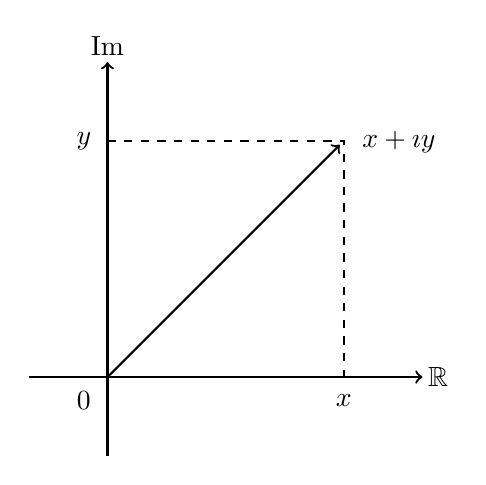
\begin{tikzpicture}
			\draw[thick, ->] (0,-1)--(0,4);
			\node at (0,4.2){Im};
			\draw[thick, ->] (-1,0)--(4,0);
			\node at (4.2,0){$\real$};
			\node at (-0.3, -0.3){0};
			%%%%%%%%%%%%%%%%%%%%%%%%%%%%%%%%
			\draw[thick, dashed] (0,3)--(3,3)--(3,0);
			\draw[thick,->] (0,0)--(2.95,2.95);
			%%%%%%%%%%%%%%%%%%%%%%%%%%%%%
			\node at (-0.3, 3){$y$};
			\node at (3,-0.3){$x$};
			\node at (3.7,2.98){$x+\imaginary y$};
		\end{tikzpicture}\caption{The geometrical representation of complex plane}\label{fig:1_1}
	\end{figure}
	Complex numbers have no real representation in the physical world, but yet they are extremely useful tools in performing calculations that have bearing in the real world. The most useful application for complex numbers is the fact they can be geometrically presented on a 2-dimensional plane and they have capability of incorporating two different values into a single vector that can be use to perform different computations.\\
	
	\NI In the field of physics, engineering, where in some cases a single number needs to represent multiple values, complex numbers show themselves to be useful because one can use a single calculation to deal with 2-dimensional problem.
	
	\section{Basic Operations with Complex Numbers}
	\subsection{Complex Numbers Algebra}
	A number such as $6+2\imaginary$ is called a complex number. It is the sum of two terms (each of which may be zero).\\
	
	\NI The Real term or is known as the real part and the coefficient of $\imaginary$ is the imaginary part. Therefore the real part of $6+2\imaginary$ is 6 and the imaginary part is 2.\\
	
	\NI Having introduced a complex number, the ways in which they can be combined i.e addition, multiplication, division etc. need to be defined. This is called or termed the \ubt{algebra} of complex numbers. As we progress, we will see that in general, $\imaginary^2 = -$ can be used where appropriate.
	
	\subsection{Additional and Subtraction of Complex Numbers}
	\ubt{Addition} of complex numbers is defined by separately adding real and imaginary parts. The parentheses do not change the problem. Combine like terms (real with real and imaginary with imaginary) by combining coefficients, so if
	\begin{equation}
		z=a+b\imaginary, p=c+d\imaginary\label{eq:1_11}
	\end{equation}
	then
	\begin{equation}
		z+p = (a+c) + (b+d)\imaginary\label{eq:1_12}
	\end{equation}
	Similarly for subtraction.
	\example{}
	Express $(7+6\imaginary) + (8-3\imaginary)$ in the form $x+y\imaginary$
	\solution
	Given\\
	$(7+6\imaginary) + (8-3\imaginary) = 7+8+(6-3)\imaginary = 15+3\imaginary$\\
	Similarly, if we have\\
	$(7+6\imaginary) - (8-3\imaginary)\implies (7-8) - (6-3)\imaginary = -1-3\imaginary$
	
	\subsection{Multiplication}
	When multiplying two complex numbers, you are just using the distributive property multiple times. Simplify the resulting expression and remember that $\imaginary^2 = -1$
	\begin{eqnarray*}
		(a+\imaginary b)(c+\imaginary d) &=& ac + a(\imaginary d)+(\imaginary d)c + (\imaginary b)(\imaginary d)\\
		&=& ac + \imaginary ad + \imaginary bc - bd ~~~ (\imaginary^2 = -1)\\
		&=& ac - bd + \imaginary(ad + bc)
	\end{eqnarray*}
	\example{}
	\begin{eqnarray*}
		(2+3\imaginary)(3+2\imaginary) &=& 2\times 3 + 2\times 2\imaginary + 3\imaginary\times 3 + 3\imaginary \times 2\imaginary\\
		&=&6 + 4\imaginary + 9\imaginary - 6 ~~~ (\imaginary^2 = -1)\\
		&=&13\imaginary
	\end{eqnarray*}
	
	\subsection{Complex Conjugation}
	For any complex number,
	\begin{equation}
		z=a+\imaginary b\label{eq:1_13}
	\end{equation}
	we define the complex conjugate to be
	\begin{equation}
		z^{*} = a-\imaginary b\label{eq:1_14}
	\end{equation}
	It is very useful since the following are real:
	\begin{eqnarray*}
		z+z^{*}&=&a+\imaginary b + (a-\imaginary b) = 2a\sps
		zz^{*} &=&(a+\imaginary b)(a-\imaginary b) = a^2 + \imaginary ab - \imaginary ab - a^2 - (\imaginary b)^2\\
		&=& a^2 + b^2
	\end{eqnarray*}
	The modulus of a complex number is defined as 
	\begin{equation}
		|z| = \sqrt{zz^{*}}
	\end{equation}
	Hence, complex conjugate of a complex number is obtained by change the sign of the imaginary part.
	\example{}
	If $z=3+2\imaginary$, $z^{*}$(conjugate)$=3-2\imaginary$
	
	\subsection{Division}
	To divide complex numbers is to multiply top and bottom by the complex conjugate of the denominator.
	\begin{eqnarray*}
		\frac{z_1}{z_2} = \frac{z_1}{z_2}= \frac{z_1}{z_2} \times \frac{z^{*}_2}{z^{*}_2} = \frac{z_1z^{*}_2}{z_2z^{*}_2}
	\end{eqnarray*}
	\example{}
	\begin{eqnarray*}
		\frac{1}{\imaginary} &=&\frac{1}{\imaginary} \times \frac{-\imaginary}{-\imaginary}\sps
		&=&\frac{-\imaginary}{\imaginary\times(-\imaginary)}\sps
		&=& \frac{-\imaginary}{1}33
		= -\imaginary		
	\end{eqnarray*}
	Similarly,
	\begin{eqnarray*}
		\frac{(2+3\imaginary)}{(1+2\imaginary)} &=& \frac{(2+3\imaginary)(1-2\imaginary)}{(1+2\imaginary)(1-2\imaginary)}\sps
		&=&\frac{(2+3\imaginary)(1-2\imaginary)}{1+4}\sps
		&=&\frac{1}{5}\Big(2+3\imaginary\Big)\Big(1-2\imaginary\Big)\sps
		&=&\frac{1}{5}\Big(2-4\imaginary+3\imaginary+6\Big)
		= \frac{1}{5}\Big(8-\imaginary\Big)
	\end{eqnarray*}
	
	\section{Solving Equations}
	Just as we have equations with real number, we can have equations with complex numbers, let us look at an example.\\
	If $4+5\imaginary = z - (1-\imaginary)$\\
	We have, 
	\begin{eqnarray*}
		z &=& x + \imaginary y\sps
		4+5\imaginary &=& x - 1 + (y+1)\imaginary\sps
	\end{eqnarray*}
	Comparing both sides
	Real parts $\implies 4 = x -1 \implies x = 5$\sps
	Imaginary parts $\implies 5 = y+1 \implies y = 4$\\
	Hence, $z = 5+4\imaginary$
	
	%%%%%%%%%%%%%%%%%%%CHAPTER TWO%%%%%%%%%%%%%%%%%%%
	\chapter{INTRODUCTION TO ANALYTIC FUNCTIONS}
	In this chapter, we shall introduce the main topic, namely the analytic functions. We shall, however, start by first introducing the complex differentiable functions.
	
	\section{Complex Differentiable Functions and Analytic Functions}
	The definition of complex differentiability of a complex function is formally identical with the definition of real differentiability, and yet there is a fundamental difference between the two definitions, which will give the complex continuously differentiable functions much better properties than the real continuously differentiable function. Therefore, one should not be confused that the definition below is just the same as the definition of real differentiability.
	
	\begin{definition}
		Let $\Omega$ be an open and non-empty subset of $\complex$ and let $f:\Omega\rightarrow\complex$ be a complex function on $\Omega$. The function $f$ is complex differentiable at a point $z_0\in\Omega$, if the limit
		\begin{equation}
			\lim\limits_{z\rightarrow z_0}\frac{f(z)-f(z_0)}{z-z_0}\label{eq:2_1}
		\end{equation} 
		exist. If this is the case, we denote this limit by 
		\begin{equation}
			f\sprime(z_0), \text{ or } \frac{df}{dz}\big(z_0\big) \text{ or } \frac{df}{dz} \text{ or } f\sprime \label{eq:2_2}
		\end{equation}
		If $f$ is complex differentiable at $z_0$, then it follows the limit expression above that that $f(z)\rightarrow f(z_0)$ for $z\rightarrow z_0$ in $\Omega$. Thus $f$ is continuous at $z_0$.
	\end{definition}
	\NI That the complex differentiability is fairly strong property - stronger than real differentiability - follows from the facts that the limit expression above does not follow a specified direction as in the real case, whereby changing the notation to real $x$, either $x\rightarrow x_0$ from below or $x\rightarrow x_0$ from above, and no other possibility.
	
	\section{Limits and Continuous Functions}
	\begin{definition}
		If $f(z)$ is defined on a punctured disk around $z_0$ or neighbourhood of $z_0$, then we say that
		\begin{equation}
			\lim\limits_{z\rightarrow z_0} f(z) = w_0\label{eq:2_3}
		\end{equation}
		If $f(z)$ goes to $w_0$ no matter what direction $z$ approaches $z_0$ .i.e the limit must be independent of the manner which $z\rightarrow z_0$.\\
	\end{definition}

	\example{}
	Many functions have obvious limits, e.g
	\begin{eqnarray*}
		\lim\limits_{z\rightarrow 2} z^2 = 4
	\end{eqnarray*}
	and
	\begin{eqnarray*}
		\lim\limits_{z\rightarrow 2} (z^2+2)/(z^3+) = \frac{6}{9}
	\end{eqnarray*}
	Here is an example of the limit that doesn't exist because different sequences give different limits.
	\example{}
	Show that
	\begin{eqnarray*}
		\lim\limits_{z\rightarrow 0}\frac{z}{\zbar} = \lim\limits_{z\rightarrow 0} \frac{x+\imaginary y}{x - \imaginary y} \text{ ~~~~~~~does not exist}
	\end{eqnarray*}
	\solution
	On the real axis, we have $y=0$
	\begin{eqnarray*}
		\frac{z}{\zbar} = \frac{x}{x} = 1
	\end{eqnarray*}
	So the limit as $z-\rightarrow 0$ along the real axis is $1$. \\
	By contrast, on the imaginary axis, we have $x=0$
	\begin{eqnarray*}
		\frac{z}{\zbar} = \frac{\imaginary y}{-\imaginary y} = -1
	\end{eqnarray*}
	So the limit as $z\rightarrow$ along the imaginary axis is $-1$. Since the two limits do not agree the limit as $z\rightarrow 0$ does not exist.
	
	\subsection{Properties of Limits}
	We have the usual properties of limits, suppose
	\begin{eqnarray}
		\lim\limits_{z\rightarrow z_0} f(z) = w_1 \text{ and } \lim\limits_{z\rightarrow z_0} g(z) = w_2
	\end{eqnarray}
	then,
	\begin{itemize}
		\item $\lim\limits_{z\rightarrow z_0} f(z) + \lim\limits_{z\rightarrow z_0} g(z) = w_1 + w_2 $
		\item $\lim\limits_{z\rightarrow z_0} f(z)g(z) = w_1 \cdot w_2$
		\item If $w_2 \neq 0$ then $\lim\limits_{z\rightarrow z_0} f(z)/g(z) = w_1/w_2$
	\end{itemize}
	
	\section{Continuous Functions}
	A function f(z) is continuous if it doesn't have any sudden jumps. Let $f(z)$ be defined and single valued in a neighbourhood of $z=z_0$ as well at $z=z_0$ the function $f(z)$ is said to be continuous at $z=z_0$ if
	\begin{eqnarray}
		\lim\limits_{z\rightarrow z_0} f(z) = f(z_0)\label{eq:2_5}
	\end{eqnarray}
	The above definition implies that the following three conditions must be satisfied for a function $f(z)$ to be continuous at $z=z_0$
	\begin{enumerate}
		\item $\lim\limits_{z\rightarrow z_0} f(z)$ must exist
		\item $f(z_0)$ must also exist
		\item $L = f(z_0)$
	\end{enumerate}
	
	\subsection{Properties of Continuous Function}
	Since continuity is defined in terms of limits, we have the following properties of continuous functions. Suppose $f(z)$ and $g(z)$ are continuous on a region $A$. Then,
	\begin{enumerate}
		\item $f(z)+g(z)$ is continuous on $A$.
		\item $f(z)g(z)$ is continuous on $A$.
		\item $f(z)/g(z)$ is continuous on $A$ except at points where $g(z)=0$.
		\item If $h$ is continuous on $f(A)$ then $h(f(z))$ is continuous on $A$.
	\end{enumerate}

	\section{Analytic Functions of a Complex Variable}
	A function $f(z)$ is said to be analytic in a region $\real$ of the complex plane if $f(z)$ has a derivative at each point of $\real$ and if $f(z)$ is single valued. Also, we can defined a function $f(z)$ to be analytic at a point $z$ if $z$ is an interior point of some region where $f(z)$ is analytic. The basic of analytic function at a point implies that the function is analytic in some circle with center at this point. The terms \ubt{Regular} and holomophic are sometimes use for synonyms for analytic.\\
	
	\NI A function $f(z)$ is said to be analytic at a point $z_0$ if there exists a neighbourhood $|z-z_0|< \delta$ at all points of which $f\sprime(z)$ exist.
	
	\example{}
	Find the derivative of $w=f(z)$ where KKK is given $z^3-2z$ at the point where (a)$z=z_0$ (b)$z=-1$
	\solution
	\begin{enumerate}
		\renewcommand{\labelenumi}{(\alph{enumi})}
		\item 	By the definition of analytic function, the derivative at $z=z_0$
		\begin{eqnarray*}
			f\sprime(z) &=&\lim\limits_{\Delta z\rightarrow 0} \frac{(f(z_0) + \Delta z) - f(z_0)}{\Delta z}\sps
			&=&\lim\limits_{\Delta z\rightarrow 0}\frac{(z_0+\Delta z)^3 - 2(z_0+\Delta z)-(z_0^3-2z_0)}{\Delta z}\sps
			&=& \lim\limits_{\Delta z\rightarrow 0} \frac{z^3+3(z_0)^2\Delta z + 3(z_0)(\Delta z)^2 + (\Delta z)^3 -2\Delta z - z_0^3}{\Delta z}\sps
			&=&\lim\limits_{\Delta z\rightarrow 0}\frac{3z^2 + 3z_0(\Delta z)^2 + (\Delta z)^3 - 2\Delta z}{\Delta z}\sps
			f\sprime(z_0) = 3z_0^2 - 2
		\end{eqnarray*}
		In general $f\sprime(z_0)= 3z^2_0 -2$ for all $z$
		\item From (a), we find that if $z_0=-1$, then
		\begin{eqnarray*}
			f\sprime(-1) = 3(-1)^2 - 2 = 3-2 = 1
		\end{eqnarray*}
	\end{enumerate}
	\begin{theorem}
		If $f(z)$ is analytic at a point $z$, then the derivative $f\sprime(z)$ is continuous at $z$.
	\end{theorem}
	\begin{corollary}
		If $f(z)$ is analytic at a point $z$, then $f(z)$ has continuous derivative of all order at the point $z$.
	\end{corollary}
	
	\section{Conditions for a Complex Functions to be Analytic}
	\subsection{A necessary condition for a complex function to be analytic}
	Let 
	\begin{eqnarray}
		f(x,y) = U(x,y) + \imaginary V(x,y)
	\end{eqnarray}
	be a complex function. Since
	\begin{eqnarray}
		x&=&\frac{(z+\zbar)}{2}\\
		&\text{and}\notag\\
		y&=&\frac{(z-\zbar)}{2}
	\end{eqnarray}
	Substituting for $x$ and $y$, we obtain,
	\begin{eqnarray}
		f(z,\zbar) = U(x,y) + \imaginary V(x,y)
	\end{eqnarray}
	A necessary condition for $f(z,\zbar)$ to be analytic is
	\begin{eqnarray}
		\frac{\partial f}{\partial z} = 0\label{eq:2_10}
	\end{eqnarray}
	Therefore, a necessary condition for $f=U+\imaginary V$ to be analytic is that $f$ depends only on $z$. In terms of the real and imaginary parts. $U,V$ of $f$, condition \refx{2_10} is equivalent to 
	\begin{eqnarray}
		\frac{\partial U}{\partial x} = \frac{\partial V}{\partial y}\label{eq:2_11}\sps
		\frac{\partial U}{\partial y} = -\frac{\partial V}{\partial x}\label{eq:2_12}
	\end{eqnarray}
	Equations \refx{2_11} and \refx{2_12} are known as the Cauchy-Riemann Equations. They are necessary condition for $f=U+\imaginary V$ to be analytic.The functions $U(x,y)$ and $V(x,y)$ are sometimes called conjugate function.
	
	\subsection{A necessary and sufficient conditions for a Complex Function to be Analytic}
	The necessary and sufficient conditions for a function $f=U+\imaginary V$ to be analytic are that
	\begin{enumerate}
		\item The four partial derivatives of its real and imaginary parts $\dsp\frac{\partial U}{\partial x},\frac{\partial V}{\partial y}, \frac{\partial U}{\partial y}, \frac{\partial V}{\partial x}$ satisfy the Cauchy-Riemann equations \refx{2_11} and \refx{2_12}.
		%%%%%%%%%%%%%%%%%%%%%
		\item The four partial derivatives of its real and imaginary parts $\dsp\frac{\partial U}{\partial x},\frac{\partial V}{\partial y}, \frac{\partial U}{\partial y}, \frac{\partial V}{\partial x}$ are continuous. Since the partial derivatives in \refx{2_11} and \refx{2_12} are continuous in $\real$, then the Cauchy-Riemann equation are sufficient condition that $f(z)$ be analytic in $\real$.
	\end{enumerate}
	
	\begin{theorem}
		If $f(z)$ is analytic, then
		\begin{eqnarray}
			\frac{\partial^2 U}{\partial x^2} + \frac{\partial^2 U}{\partial y^2} = 0\label{eq:2_13}\sps
			%%%%%%%%%%%%%%%
			\frac{\partial^2 V}{\partial x^2} + \frac{\partial^2 V}{\partial y^2} = 0\label{eq:2_14}
		\end{eqnarray}
	\end{theorem}
	If the real and imaginary parts of an analytic function are harmonic conjugate functions i.e solutions to Laplace equation and satisfy the Cauchy-Riemann equations. As we have seen, if the second partial derivatives of $U$ and $V$ with respect to $x$ and $y$ exists and continuous in a region $\real$.
	
	\section{Singularities of Analytic Functions}
	Points at which a function $f(z)$ is not analytic are called singular points or singularities of $f(z)$. There are two different types of singular points.
	
	\subsection{Isolated Singular Points}
	If $f(z)$ is analytic everywhere throughout some neighbourhood of a point $z=a$, say inside a circle $\complex:|z-a|=\real$ except at the point $z=a$, itself, then $z=a$ is called an isolated singular point of $f(z)$. $f(z)$ cannot be bounded near an isolated singular point.
	
	\subsubsection{Poles}
	If $f(z)$ has an isolated singular point at $z=a$ i.e $f(z)$ is not finite at $z=a$ and if in addition there exists an integer $n$ such that the product
	\begin{eqnarray}
		(z-a)^n f(z)
	\end{eqnarray}
	is analytic at $z=a$, then $f(z)$ has a pole of order $n$ at $z=a$, if $n$ is the smallest such integer. Note that because $(z-a)^nf(z)$ is analytic at $z=a$, such a singularity is called a removable singularity. 
	\example{}
	$\dsp f(z)= \frac{1}{(1-z)^2}$ it has a pole of 2 at $z=0$.
	
	\subsection{Essential Singularities}
	A singular point $z_0$ of $f(z)$ is called essential if it is not classifiable as any pole, removable or branch point. E.g $f(z)\sin\left(\frac{1}{2}\right)$ has an essential singularity at $z=0$.
	
	\subsection{Branch Points}
	When $f(z)$ is multivalued function, any point which cannot be an interior point of the region of definition of a single-valued branch of $f(z)$ is a singular branch point.
	\example{}
	$\dsp f(z)=\sqrt{z-a}$ has a branch point at $z=a$
	
	
	
	
	
	
	
	
	
	
	
	
	
	
	
	
	
	
	
	
	
	
	
	
	
	
	
	
	
	
	
	
	
	
	
	
	
	
	
	
	
	
	
	%%%%%%%%%%%%%%%%%%%CHAPTER THREE%%%%%%%%%%%%%%%%%%%
	\chapter{THE GAMMA FUNCTION}
	
	

	
	%%%%%%%%%%%%%%%%%%%CHAPTER FOUR%%%%%%%%%%%%%%%%%%%
	\chapter{ANALYTICAL APPLICATIONS OF THE GAMMA FUNCTION}
	


	
	%%%%%%%%%%%%%%%%%%%CHAPTER FIVE%%%%%%%%%%%%%%%%%%%
	\chapter{SUMMARY, CONCLUSION AND RECOMMENDATION}
	\section{Summary}
	In this project, the chapter one (1) tells the about complex number in various field. We have learnt that complex number is denoted as $\complex$ and it consist of two parts(the real and imaginary). Complex number arises as a result of negative value in a square root, most especially when working or solving quadratic equation. Cardano was able to crack what had seemed to be impossible task of solving the general cubic equation.\\
	
	\NI In Chapter two (2), we studied the analytic functions. A function is said to be analytic if it is differentiable at a point.\\
	
	\NI Thirdly, in chapter three of this project, we made research on Laurent series, how it is being originated by providing the theorem.\\
	
	\NI Lastly, In chapter four (4), we looked at practical problems and how it can be solved using the Laurent series expansion. We were able to use Laurent series of function about some fixed points in the their region to solve all the problems.
	\section{Conclusion}
	The Gamma function has been studied and presented 
	

	
	%%%%%%%%%%%%%%%%%%%REFERENCE%%%%%%%%%%%%%%%%%%%
	\chapter*{REFERENCES}
	\addcontentsline{toc}{chapter}{REFERENCES}
	
	\begin{description}
		\item J
		
	\end{description}
	
\end{document}